% 9 variables in here:
% h_1 = 10.0, h_2 = 10.0, h_3 = 10.0, ux_1 = 0.0, ux_2 = 1.0, ux_3 = 0.0, uy_1 = 0.0, uy_2 = 1.0, uy_3 = 0.0
\begin{figure}[ht]
\centering
  \subfigure[] {
    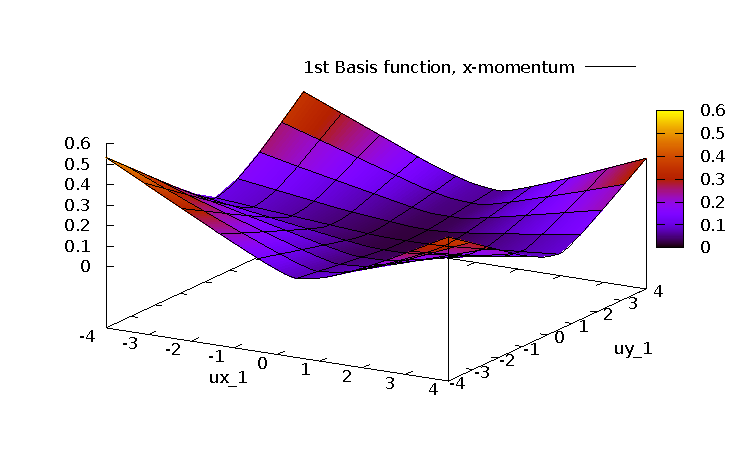
\includegraphics[scale=\zoomfactor]{{{ord1_varying_ux1_uy1_differing_ux2_uy2_1_1/10.0_10.0_10.0_x_1.0_0.0_y_1.0_0.0f00}}}
  }
  \subfigure[] {
    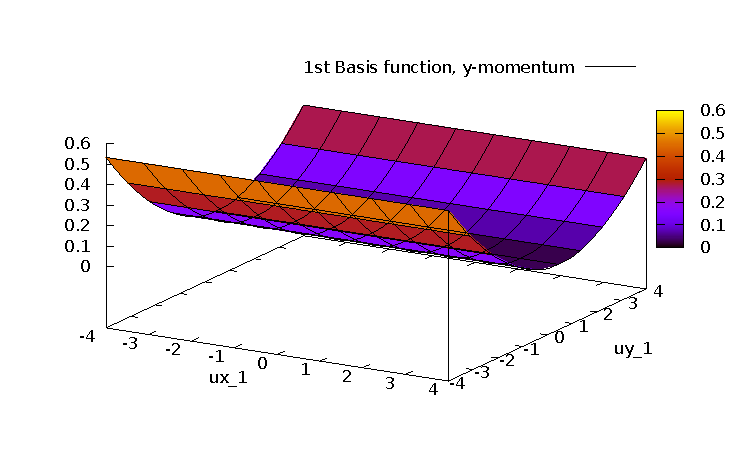
\includegraphics[scale=\zoomfactor]{{{ord1_varying_ux1_uy1_differing_ux2_uy2_1_1/10.0_10.0_10.0_x_1.0_0.0_y_1.0_0.0f01}}}
  }
  \subfigure[] {
    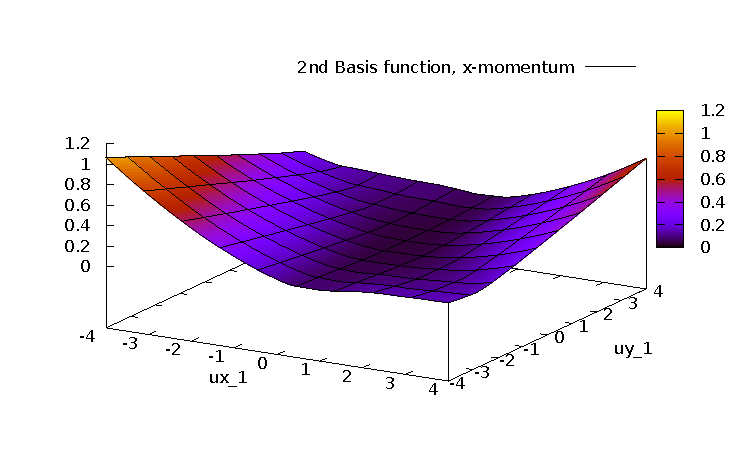
\includegraphics[scale=\zoomfactor]{{{ord1_varying_ux1_uy1_differing_ux2_uy2_1_1/10.0_10.0_10.0_x_1.0_0.0_y_1.0_0.0f02}}}
  }
  \subfigure[] {
    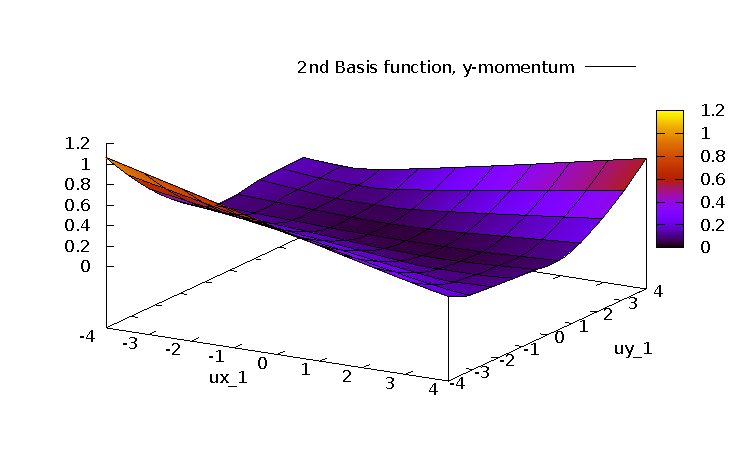
\includegraphics[scale=\zoomfactor]{{{ord1_varying_ux1_uy1_differing_ux2_uy2_1_1/10.0_10.0_10.0_x_1.0_0.0_y_1.0_0.0f03}}}
  }
  \subfigure[] {
    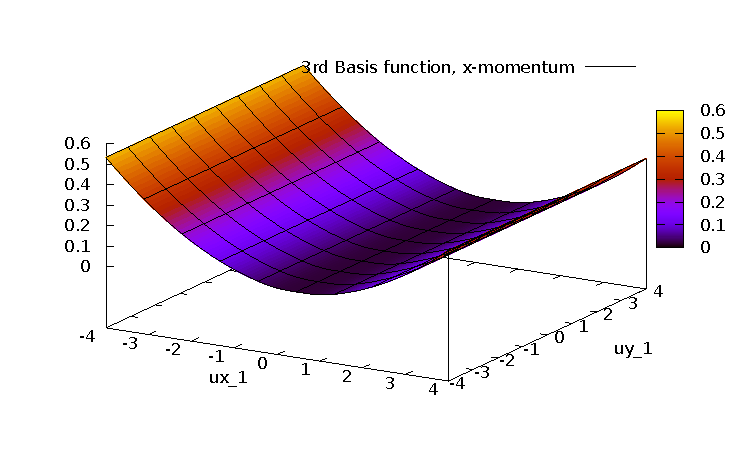
\includegraphics[scale=\zoomfactor]{{{ord1_varying_ux1_uy1_differing_ux2_uy2_1_1/10.0_10.0_10.0_x_1.0_0.0_y_1.0_0.0f04}}}
  }
  \subfigure[] {
    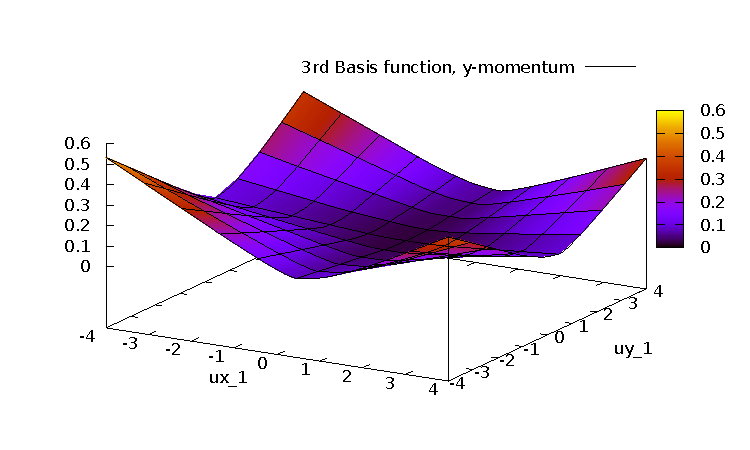
\includegraphics[scale=\zoomfactor]{{{ord1_varying_ux1_uy1_differing_ux2_uy2_1_1/10.0_10.0_10.0_x_1.0_0.0_y_1.0_0.0f05}}}
  }
\caption{}
\label{fig:ord1_varying_ux1_uy1_differing_ux2_uy2_1_1}
\end{figure}
